\section{La reconnaissance faciale}
%\textit{Présentation de qqes résultats fondamentaux sur des recherches en cognition et reconnaissance faciale du visage}
La reconnaissance faciale est une des techniques utilisables dans les systèmes biométriques d'authentification \textit{(ex: contrôle d'accès)} ou d'identification \textit{(ex: surveillance d'un lieu)}.
\\
Plusieurs méthodes peuvent être appréhendées pour la capture de l'image, cela va dépendre principalement du contexte: il peut s'agir d'un système statique ou bien dynamique, d'une reconnaissance 2D ou 3D, ... Les capteurs de l'information et les algorithmes doivent être choisis en conséquence.

\subsection{Détection de visage}
Après avoir capturé la donnée à analyser, dans ce cas-ci une image ou une vidéo, la première étape consiste à en extraire l'information utile. Plusieurs méthodes permettent de détecter des visages dans une image, elles peuvent être regroupées en quatre catégories \cite{Xthesis_1}
\begin{enumerate}
\item \textit{Knowledge-based methods}: basées sur la connaissance des éléments caractéristiques d'un visage (\textit{nez, bouche, yeux,...}) et des relations entre eux, pour déterminer si les positions relatives décrivent un visage ou non. Malheureusement, ces techniques ont un faible taux de détection.
\item \textit{Feature invariant approaches}: basées sur des éléments invariants tels que la signature de couleur de peau ou les caractéristiques du visages. Un algorithme classique est celui de \textit{De Silva} qui consiste à trouver l'axe des yeux et utiliser ensuite comme référence la longueur entre le haut du visage et le plan de l'oeil.
\item \textit{Template matching methods}: basées sur l'utilisation de templates pour calculer la corrélation entre l'image candidate et un template. Un modèle est défini à partir d'un certains nombre de relations "essentielles" et "de confirmation". Un visage est alors localisé lorsque le nombre de relations détectées dépasse un certain seuil.
\item \textit{Appearance-based methods}: basées sur la connaissance de modèles obtenus par apprentissage automatique. On retrouve ici un algorithme fréquemment utilisé, celui de \textit{Viola et Jones}, qui utilise un nombre considérable de modèles exemples représentants la variabilité de l'aspect facial. Il analyse l'image de façon itérative, en agrandissant sa fenêtre de recherche en pixels, pour y retrouver des visages.
\end{enumerate}
\paragraph{}
Plusieurs difficultés se présentent lors de cette étape et compliquent la localisation du visage. En effet, les conditions de capture de l'image peuvent varier, les éléments suivants rentrent donc en compte:
%il n'est pas toujours garantit d'obtenir 
\begin{itemize}
\item[$\cdot$]la \textit{pose}: fait varier l'orientation du visage
\item[$\cdot$]les \textit{occultations}: le visage peut être partiellement ou complètement caché par certains objets
\item[$\cdot$]les \textit{expressions faciales}: engendrent la déformation du visage et donc des variations des positions des éléments caractéristiques
\item[$\cdot$]la \textit{luminosité}: les conditions d'éclairage et les ombres qui en résultent peuvent affecter l'aspect du visage.
\item[$\cdot$]la \textit{présence ou absence de composantes structurales}: telles que la barbe, la moustache, les lunettes,...
\end{itemize}

\subsection{Prétraitement ou normalisation}
Une fois le visage détecté dans l'image, l'étape de prétraitement va permettre de rendre cette photo exploitable en la ramenant à un format prédéfini. Ainsi, toutes les images auront une taille, une échelle et des couleurs normalisées, ce qui est essentiel pour garantir les performances de la reconnaissance \cite{Xthesis_1}.
\\
Deux processus sont importants pour préparer l'image:
\begin{enumerate}
\item normalisation \textsc{géométrique}: permet de positionner et redimensionner la taille du visage
\item normalisation \textsc{photométrique}: consiste à jouer sur les niveaux de l'illumination du visage, par exemple, en augmentant les nuances pour améliorer le contraste.
\end{enumerate}


\subsection{Reconnaissance 2D}
L'étape de reconnaissance permet d'extraire de l'image les informations qui serviront à la création d'une signature numérique et, par la suite, à la comparaison avec les modèles en BDD.
Les techniques qui permettent la reconnaissance de données à partir d'une image 2D peuvent être regroupées en trois familles \cite{Xphdthesis_1}
\begin{enumerate}\setlength{\itemsep}{.3em}
\item Approches \textsc{\textbf{globales}}: le visage tout entier est utilisé et représenté par un vecteur de grande dimension.
\\L'avantage de ces méthodes est qu'elles permettent de conserver toutes les informations du visage et peuvent donc tenir compte des aspects de l'organisation globale de celui-ci. 
\\Cependant, elles utilisent uniquement des images 2D, qui sont d'autant plus sensibles aux critères cités précédemment (\textit{pose, illumination, expression,...}), et l'espace occupé par ces vecteurs est assez contraignant. \paragraph{}Il est alors possible d'utiliser des techniques de réduction de la dimension, telles que:
	\begin{itemize}\setlength{\itemsep}{.3em}
	\item[$\cdot$]\textit{\textbf{A}nalyse en \textbf{C}omposantes \textbf{P}rincipales (ACP)}: dont une des méthodes les plus utilisées est l'\textit{Eigenfaces} qui calcule les propriétés du visage à partir de combinaisons de vecteurs propres issus des modèles dans différentes nuances de gris.
	\item[$\cdot$]\textit{\textbf{A}nalyse \textbf{D}iscriminante \textbf{L}inéaire (ADL)}: une amélioration de la précédente.
	\end{itemize}
\item Approches \textsc{\textbf{locales}}: le visage est ici représenté par un ensemble de vecteurs de dimensions plus faibles. Il existe deux grandes catégories de techniques:
	\begin{itemize}
	\item[$\cdot$] \textit{basées sur les point d'intérêts}: les méthodes consistent à identifier des points particuliers du visage pour ensuite en déterminer les caractéristiques. Une technique reconnue est l'\textit{\textbf{E}lastic \textbf{B}unch \textbf{G}raph \textbf{M}atching (EBGM)} qui consiste à créer un réseaux pour modéliser les relations entre les points d'intérêts. On obtient ainsi un graphe topologique (fig \ref{graphe-topo}).

	\item[$\cdot$] \textit{basées sur l'apparence du visage}: le visage est divisé en plus petites régions, desquelles on extrait les caractéristiques locales.
	\end{itemize}
\item Approches \textsc{\textbf{hybrides}}: techniques qui utilisent les caratéristiques locales et globales.
	\begin{figure}[h!]
	\center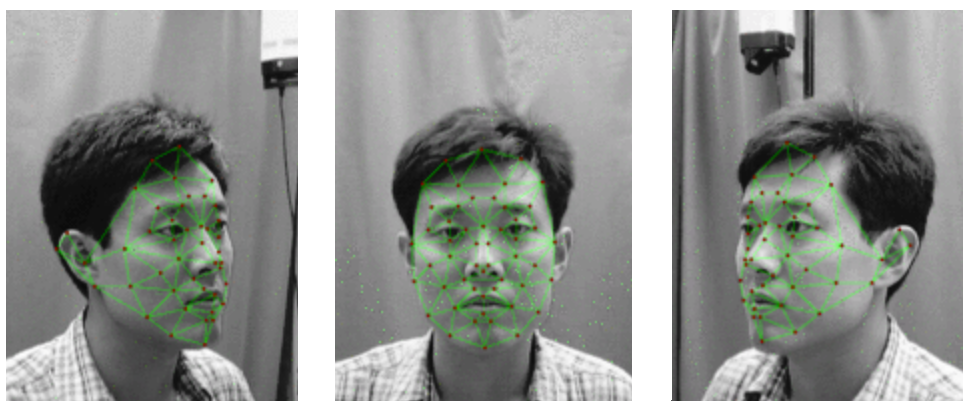
\includegraphics[scale=.3]{images/ebgm}\label{graphe-topo}
	\caption{Graphe topologique par EBGM \cite{Ximage_1}}
	\end{figure}
\end{enumerate}

De manière générale, les méthodes locales sont plus performantes et surtout moins sensibles aux changements de l'environnement, qui surviennent lors de la capture d'image (voir annexe \ref{locales-vs-globales}).


%\textit{Exploitation des caractéristiques extraites, création d'une signature numérique et mise en correspondance avec les modèles de la DB ou le modèle est vérifié\paragraph{}
%Difficultés: causes inter-sujets (ressemblance entre modèles) et intra-sujet (ci-dessus)}

\subsection{Reconnaissance 3D}
Contrairement aux techniques 2D qui viennent d'être présentées, les technologies de reconnaissance 3D permettent d'introduire la notion de \textit{profondeur} dans les images analysées. De telles techniques sont en plein essors et très prometteuses quant à leurs performances.
\\
Si les méthodes de reconnaissance sont différentes de la 2D, il en va de même pour les informations traitées et donc pour les capteurs utilisés qui ne sont plus de simples caméras. 
\\En effet, pour reconstruire un visage en 3D (\textit{par maillage polygonal par exemple}), un matériel spécial est nécessaire tel que des caméras à vision stéréoscopique ou des scans 3D à vision active. La première catégorie utilise plusieurs caméras qui sont positionnées à des endroits bien spécifiques par rapport à des jeux de lumières. Tandis que les scans projettent des rayons de lumière et détectent par caméra les courbes formées sur le visage.
\begin{figure}[h!]
\center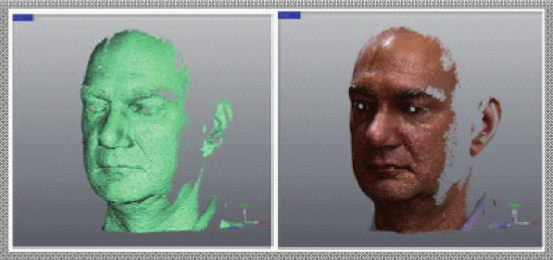
\includegraphics[scale=.35]{images/scans-3D}
\caption{Scans 3D \textit{sans} et \textit{avec} mapping de texture. Modèles issus de la base FRGCv2 \cite{Xphdthesis_4}}
\end{figure}\\
Les principales méthodes actuelles qui permettent la reconnaissance de visages en 3D sont les suivantes \cite{Xphdthesis_4}:
\begin{itemize}\setlength{\itemsep}{.2em}
\item[$\cdot$]Approches \textsc{\textbf{surfaces}}: la surface 3D du modèle reconstruit est alignée avec celle de la signature à comparer pour évaluer le taux de similitude par approximations.
\item[$\cdot$]Approches \textsc{\textbf{holistiques}} ou (\textsc{globales}): extensions des méthodes ACP 2D pour les représentations 3D, par exemple: \textit{eigensurfaces}.
\item[$\cdot$]Approches \textsc{\textbf{locales}}: cherchent des courbes du visages ou des points caractéristiques
\item[$\cdot$]Approches \textsc{\textbf{3D + 2D}}: combinaisons de techniques d'analyse 3D et 2D pour améliorer les performances et la robustesse
\end{itemize}
\paragraph{}
La reconnaissance 3D comparée à la 2D permet d'obtenir de meilleurs résultats.
\\
De plus, les scans 3D sont beaucoup moins sensibles aux divers changements d’illumination, de variation de la pose ou encore de mise à l’échelle, autant de critères qui sont les éléments critiques de la reconnaissance automatique 2D.
\\
Toutefois, elle est plus difficile à mettre en place, consomme plus de ressources de calcul et nécessite l'utilisation de capteurs plus onéreux.

\subsection{Identification et authentification}\label{id-vs-auth}
Une fois la signature reconstruite à partir des données extraites de l'image, celle-ci va être comparée avec d'autres signatures. La validation se base sur un seuil du taux de similitudes entre les deux fichiers numériques.
\paragraph{}Dans le cas de l'identification, la signature peut être comparée avec l'ensemble des gabarits de la BDD pour retrouver l'individu en question ou, dans une optique de recherches, elle peut être comparée avec seulement une liste de modèles pour détecter un éventuel match.
\paragraph{}Dans une utilisation d'authentification, une requête est faite vers la BDD pour obtenir le modèle à comparer et vérifier si la signature reconstruite y correspond ou non.
\subsection{Mesure de la performance}
Afin d'évaluer les performances d'un système biométrique par reconnaissance de visage et pour aider la recherche et le développement de ces technologies, il existe des bases de données contenant de nombreux templates pouvant être utilisés. Ainsi, à titre d'exemple, il existe la base FERET, avec plusieurs centaines d'invidus collectés, ou la base XM2VTS qui contient un ensemble d'images faciales 2D et 3D avec différentes prises de vues \cite{Xphdthesis_3}.

